\documentclass{article}
\usepackage{tikz}
\usepackage{amsmath}

\title{Probability Theory Solutions}
\author{Student}
\date{\today}

\begin{document}

\maketitle

\section*{1.1 Nubrėžkite šių įvykių Veno diagramas:}
\begin{itemize}
    \item[(a)] \( A \cap B \)
    \item[(b)] \( A \cup B \)
\end{itemize}

\subsection*{Solution:}
\begin{itemize}
    \item[(a)] \( A \cap B \) - The intersection of events A and B.
    \begin{center}
        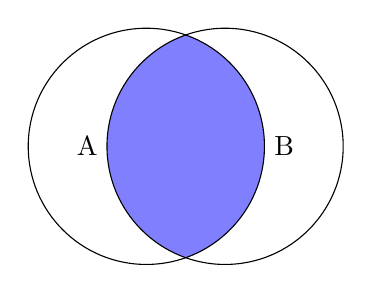
\begin{tikzpicture}
            \begin{scope}
                \clip (0,0) circle (1.5);
                \fill[blue!50] (1,0) circle (1.5);
            \end{scope}
            \draw (0,0) circle (1.5);
            \draw (1,0) circle (1.5);
            \node at (-0.75,0) {A};
            \node at (1.75,0) {B};
        \end{tikzpicture}
    \end{center}
    
    \item[(b)] \( A \cup B \) - The union of events A and B.
    \begin{center}
        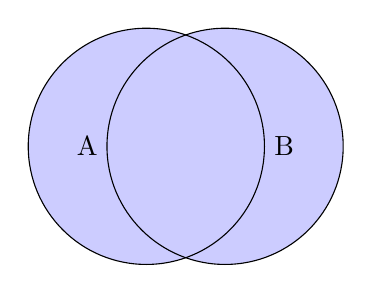
\begin{tikzpicture}
            \fill[blue!20] (0,0) circle (1.5);
            \fill[blue!20] (1,0) circle (1.5);
            \draw (0,0) circle (1.5);
            \draw (1,0) circle (1.5);
            \node at (-0.75,0) {A};
            \node at (1.75,0) {B};
        \end{tikzpicture}
    \end{center}
\end{itemize}

\section*{1.2 Given events \(A\) and \(B\), express \(A \cup B\) and \(A \cap B\) using set notation.}

\subsection*{Solution:}
\[
A \cup B = \{x \mid x \in A \text{ or } x \in B\}
\]
\[
A \cap B = \{x \mid x \in A \text{ and } x \in B\}
\]

\section*{1.3 Kada a) \(A \cap B = A\); b) \(A \cup B = A\)?}

\subsection*{Solution:}
\begin{itemize}
    \item[(a)] \(A \cap B = A\) when \(A \subseteq B\). This means that event A is entirely contained within event B.
    \item[(b)] \(A \cup B = A\) when \(B \subseteq A\). This means that event B is entirely contained within event A.
\end{itemize}

\section*{1.4 Įvykis \(A\) yra įvykio \(B\) dalis. Kam lygi jų a) sąjunga; b) sankirta?}

\subsection*{Solution:}
\begin{itemize}
    \item[(a)] Sąjunga \(A \cup B = B\) since \(A \subseteq B\).
    \item[(b)] Sankirta \(A \cap B = A\) since \(A \subseteq B\).
\end{itemize}

\section*{1.5 Determine the complement of event \(A\), denoted as \(A^C\).}

\subsection*{Solution:}
\[
A^C = \{x \mid x \notin A\}
\]

\section*{1.6 Ar įvykiai \(A\) ir \(A \cup B\) yra sutaikomi? Pagrįskite savo išvadą.}

\subsection*{Solution:}
Įvykiai \(A\) ir \(A \cup B\) nėra sutaikomi, nes \(\emptyset \ne A \cap (A \cup B) = A\). Kadangi \(A\) visada įvyksta kartu su \(A \cup B\), jie negali būti nesutaikomi.

\section*{1.7 Užrašykite įvykį \(A \setminus B\) dviem kitais būdais.}

\subsection*{Solution:}
\[
A \setminus B = A \cap B^C = A \cap \neg B
\]

\section*{1.8 Moneta metama tris kartus (i=1, 2, 3). Įvykis \(A_i\) – atvirto skaičius, įvykis \(B_i\) – atvirto herbas. Aprašykite įvykį \(C\), kad atvirto ne mažiau kaip du herbai.}

\subsection*{Solution:}
Įvykis \(C\) apibūdinamas taip: ne mažiau kaip du herbai:
\[
C = (B_1 \cap B_2) \cup (B_1 \cap B_3) \cup (B_2 \cap B_3)
\]

\section*{1.11 Describe event \(A \setminus B\) graphically using a Venn diagram.}

\subsection*{Solution:}
\begin{center}
    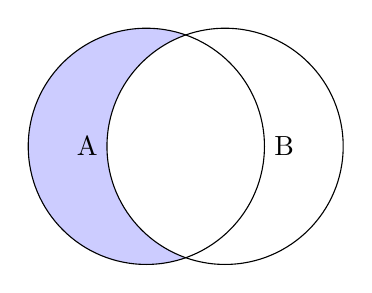
\begin{tikzpicture}
        \fill[blue!20] (0,0) circle (1.5);
        \begin{scope}
            \clip (0,0) circle (1.5);
            \fill[white] (1,0) circle (1.5);
        \end{scope}
        \draw (0,0) circle (1.5);
        \draw (1,0) circle (1.5);
        \node at (-0.75,0) {A};
        \node at (1.75,0) {B};
    \end{tikzpicture}
\end{center}

\section*{1.13 For events \(A\) and \(B\), show graphically that \(A \cap B^C = A \setminus B\).}

\subsection*{Solution:}
\begin{center}
    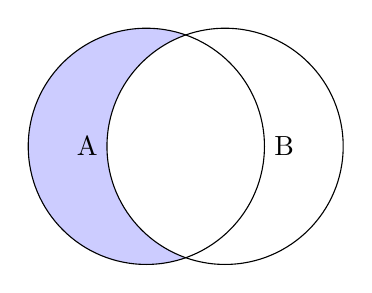
\begin{tikzpicture}
        \fill[blue!20] (0,0) circle (1.5);
        \begin{scope}
            \clip (0,0) circle (1.5);
            \fill[white] (1,0) circle (1.5);
        \end{scope}
        \draw (0,0) circle (1.5);
        \draw (1,0) circle (1.5);
        \node at (-0.75,0) {A};
        \node at (1.75,0) {B};
    \end{tikzpicture}
\end{center}
\[
A \cap B^C = A \setminus B
\]

\section*{1.14 \(A\), \(B\), ir \(C\) yra įvykiai. Užrašykite tokius įvykius:}

\subsection*{Solution:}
\begin{itemize}
    \item[(a)] \(A \cap B^C \cap C^C\)
    \item[(b)] \(A \cap B \cap C^C\)
    \item[(c)] \(A \cap B \cap C\)
    \item[(d)] \(A \cup B \cup C\)
    \item[(e)] \((A \cap B) \cup (A \cap C) \cup (B \cap C)\)
    \item[(f)] \(A^C \cap B^C \cap C^C\)
    \item[(g)] \((A \cap B^C \cap C^C) \cup (A^C \cap B \cap C^C) \cup (A^C \cap B^C \cap C)\)
    \item[(h)] \((A \cap B \cap C^C) \cup (A \cap B^C \cap C) \cup (A^C \cap B \cap C) \cup (A \cap B^C \cap C^C) \cup (A^C \cap B \cap C^C) \cup (A^C \cap B^C \cap C)\)
\end{itemize}

\section*{2.1 Dėžėje yra 3 balti ir 7 juodi rutuliai. Atsitiktinai vieną ištraukiame. Kokia tikimybė, kad jis bus baltas?}

\subsection*{Solution:}
\begin{align*}
    P(\text{baltas}) &= \frac{\text{baltų rutulių skaičius}}{\text{visų rutulių skaičius}} \\
    &= \frac{3}{3 + 7} \\
    &= \frac{3}{10}
\end{align*}
Tikimybė, kad ištrauktas rutulys bus baltas, yra \( \frac{3}{10} \) arba 0.3.

\section*{2.2 Yra 52 kortų kaladė. Atsitiktinai traukiame vieną kortą. Kokia tikimybė, kad: a) tai ne tūzas; b) ištrauktos kortos vertė bus žemesnė už septynakę?}

\subsection*{Solution:}
\begin{itemize}
    \item[(a)] 
    Tikimybė, kad tai ne tūzas:
    \[
    P(\text{ne tūzas}) = 1 - P(\text{tūzas}) = 1 - \frac{4}{52} = \frac{48}{52} = \frac{12}{13}
    \]
    \item[(b)]
    Kortos vertės, kurios yra žemesnės už septynakę: 2, 3, 4, 5, 6 (po 4 kiekvienos rūšies):
    \[
    P(\text{žemesnė už septynakę}) = \frac{20}{52} = \frac{5}{13}
    \]
\end{itemize}

\section*{2.3 Po krepšinio varžybų susumavus žaidėjo pataikymo rezultatus buvo gauta, kad jo pataikymo procentas – 60 %. Kiek kartų jis metė kamuolį, jeigu nepataikė į krepšį 12 kartų?}

\subsection*{Solution:}
Tegul \(N\) yra bendras metimų skaičius. Kadangi 60% metimų buvo taiklūs, tai 40% buvo netaiklūs. Jei žaidėjas nepataikė 12 kartų, tai:
\[
0.4N = 12
\]
\[
N = \frac{12}{0.4} = 30
\]
Taigi, žaidėjas metė kamuolį 30 kartų.

\section*{2.4 Two events \(A\) and \(B\) are independent. Express this condition in terms of probabilities.}

\subsection*{Solution:}
Events \(A\) and \(B\) are independent if and only if:
\[
P(A \cap B) = P(A) \cdot P(B)
\]

\section*{2.6 Metami 3 lošimo kauliukai. Kurio įvykio tikimybė didesnė: atvirtusių akučių suma lygi 9 ar atvirtusių akučių suma lygi 10?}

\subsection*{Solution:}
Galimi deriniai, kai suma yra 9:
\[
(1,2,6), (1,3,5), (1,4,4), (2,2,5), (2,3,4), (3,3,3)
\]
Galimi deriniai, kai suma yra 10:
\[
(1,3,6), (1,4,5), (2,2,6), (2,3,5), (2,4,4), (3,3,4)
\]

Skaičius derinių kiekvienu atveju yra 6. Kadangi abu įvykiai turi vienodą derinių skaičių, jų tikimybės yra vienodos.

\section*{2.7 In a group of 100 people, 60 like apples, 40 like bananas, and 20 like both. What is the probability that a randomly chosen person likes at least one of the two fruits?}

\subsection*{Solution:}
Using the principle of inclusion-exclusion, the number of people who like at least one of the fruits is:
\[
|A \cup B| = |A| + |B| - |A \cap B| = 60 + 40 - 20 = 80
\]

The probability that a randomly chosen person likes at least one of the fruits is:
\[
P(A \cup B) = \frac{|A \cup B|}{100} = \frac{80}{100} = 0.8
\]

\section*{2.8 In a lottery, a ticket has a probability of \(\frac{1}{1000}\) to win. What is the probability of not winning?}

\subsection*{Solution:}
The probability of not winning is the complement of winning:
\[
P(\text{not winning}) = 1 - P(\text{winning}) = 1 - \frac{1}{1000} = \frac{999}{1000}
\]

\section*{2.9 Du draugai susitarė susitikti tarp 12.00 val. ir 13.00 val. ir laukti vienas kito ne ilgiau 15 min ir ne vėliau 13.00 val. Kokia tikimybė, kad susitikimas įvyks?}

\subsection*{Solution:}
Laikas, kurį draugas gali atvykti, yra nuo 0 iki 60 minučių. Tegul \(X\) ir \(Y\) yra jų atvykimo laikai. Norėdami susitikti, atvykimo laikas turi skirtis ne daugiau kaip 15 minučių:
\[
|X - Y| \leq 15
\]

Plotas kvadrate \(60 \times 60\) yra 3600 kvadratinės minutės. Plotis susitikimo sąlygos (trikampis su dviem simetriškais trikampiais) yra:
\[
2 \cdot \frac{1}{2} \cdot 45 \cdot 45 = 2025
\]

Tikimybė:
\[
P(\text{susitikimas}) = \frac{2025}{3600} = \frac{9}{16}
\]

\section*{2.10 A box contains 5 red, 3 green, and 2 blue balls. If one ball is drawn at random, what is the probability that it is either red or blue?}

\subsection*{Solution:}
The total number of balls is:
\[
5 + 3 + 2 = 10
\]

The number of red or blue balls is:
\[
5 + 2 = 7
\]

The probability of drawing a red or blue ball is:
\[
P(\text{red or blue}) = \frac{7}{10}
\]

\section*{2.11 Atkarpoje atsitiktinai pažymimas taškas. Kokia tikimybė, kad jo atstumas iki atkarpos vidurio bus didesnis už trečdalį atkarpos ilgio?}

\subsection*{Solution:}
Tegul atkarpos ilgis yra \(l\). Atstumas nuo vidurio, didesnis už \(\frac{l}{3}\), reiškia, kad taškas yra už intervalo \(\left(\frac{l}{3}, \frac{2l}{3}\right)\).

Atstumas mažesnis nei \(\frac{l}{3}\) yra du intervalai: \(\left[0, \frac{l}{3}\right]\) ir \(\left[\frac{2l}{3}, l\right]\). Bendras ilgis:
\[
\frac{l}{3} + \frac{l}{3} = \frac{2l}{3}
\]

Tikimybė:
\[
P = \frac{\frac{2l}{3}}{l} = \frac{2}{3}
\]

\section*{2.16 Atkarpa padalinta į 5 lygias dalis. Joje atsitiktinai padedama 10 taškų. Kokia tikimybė, kad į pirmą atkarpos dalį pateko 2 taškai, į antrą – 3 taškai, į ketvirtą – 4 taškai, į penktą – 1 taškas?}

\subsection*{Solution:}
Tikimybė, kad taškai pasiskirstys būtent taip, yra:
\[
P = \frac{10!}{2!3!0!4!1!} \left(\frac{1}{5}\right)^{10} = \frac{10!}{2!3!4!1!} \left(\frac{1}{5}\right)^{10}
\]

Apskaičiuojame faktorius:
\[
P = \frac{3628800}{2 \cdot 6 \cdot 24 \cdot 1} \left(\frac{1}{5}\right)^{10} = \frac{3628800}{288} \left(\frac{1}{5}\right)^{10} = 12600 \cdot \left(\frac{1}{5}\right)^{10} = 12600 \cdot \frac{1}{9765625} \approx 0.00129
\]

Tikimybė yra 0.00129 arba 0.129%.


\section*{2.17 Dėžėje yra 10 iš eilės (nuo 1 iki 10) sunumeruotų rutulių. Atsitiktinai vieną ištraukiame. Kokia tikimybė, kad jo numeris dalijasi iš dviejų arba trijų?}
\subsection*{Solution:}
The numbers that are divisible by 2 are: 2, 4, 6, 8, 10 (5 numbers).
The numbers that are divisible by 3 are: 3, 6, 9 (3 numbers).
The number divisible by both 2 and 3 is: 6 (1 number).

Using the principle of inclusion and exclusion:
\[
P(A \cup B) = P(A) + P(B) - P(A \cap B)
\]
\[
P(\text{divisible by 2 or 3}) = \frac{5}{10} + \frac{3}{10} - \frac{1}{10} = \frac{7}{10}
\]

The probability is \( \frac{7}{10} \) or 0.7.

\section*{2.21 Sandėlyje yra 20 pirmos rūšies detalių, 6 – antros ir 4 – trečios rūšies. Kokia tikimybė, kad atsitiktinai paimtos dvi detalės yra skirtingų rūšių?}
\subsection*{Solution:}
Total number of details: \(20 + 6 + 4 = 30\)

Number of ways to choose 2 details: \(\binom{30}{2} = \frac{30 \cdot 29}{2} = 435\)

Number of ways to choose 2 details of the same type:
\[
\binom{20}{2} + \binom{6}{2} + \binom{4}{2} = \frac{20 \cdot 19}{2} + \frac{6 \cdot 5}{2} + \frac{4 \cdot 3}{2} = 190 + 15 + 6 = 211
\]

Number of ways to choose 2 details of different types:
\[
435 - 211 = 224
\]

Probability:
\[
P(\text{different types}) = \frac{224}{435} \approx 0.515
\]

\section*{2.26 Berniukas žaidžia su penkiomis raidyno raidėmis: E, I, N, R, S. Kokia tikimybė, kad atsitiktinai dėdamas jas į eilę, jis sudės žodį NERIS?}
\subsection*{Solution:}
Total permutations of 5 letters:
\[
5! = 120
\]

There is only 1 permutation that forms the word "NERIS". 

Probability:
\[
P(\text{NERIS}) = \frac{1}{120} \approx 0.0083
\]

\section*{2.33 Iš n turimų raktų spynai tinka tik vienas. Kokia tikimybė rasti tinkamą raktą a) pirmuoju; b) antruoju; c) trečiuoju bandymu (kartą pabandžius netinkamas raktas atgal negrąžinamas)?}
\subsection*{Solution:}
a) Pirmuoju bandymu:
\[
P(\text{first try}) = \frac{1}{n}
\]

b) Antruoju bandymu:
\[
P(\text{second try}) = \frac{n-1}{n} \cdot \frac{1}{n-1} = \frac{1}{n}
\]

c) Trečiuoju bandymu:
\[
P(\text{third try}) = \frac{n-1}{n} \cdot \frac{n-2}{n-1} \cdot \frac{1}{n-2} = \frac{1}{n}
\]

\section*{2.40 Metama moneta ir kauliukas. Kokia tikimybė, kad atvirs herbas ir lyginis akučių skaičius?}
\subsection*{Solution:}
Probability of flipping a head:
\[
P(\text{head}) = \frac{1}{2}
\]

Probability of rolling an even number (2, 4, 6):
\[
P(\text{even}) = \frac{3}{6} = \frac{1}{2}
\]

Combined probability:
\[
P(\text{head and even}) = P(\text{head}) \times P(\text{even}) = \frac{1}{2} \times \frac{1}{2} = \frac{1}{4}
\]

\section*{2.53 Kokia tikimybė, kad iš kaladės ištraukus 5 kortas bus bent vienas tūzas?}
\subsection*{Solution:}
Probability of not drawing an ace in one draw:
\[
P(\text{not ace}) = \frac{48}{52} = \frac{12}{13}
\]

Probability of not drawing an ace in 5 draws:
\[
P(\text{no aces in 5 draws}) = \left(\frac{12}{13}\right)^5
\]

Probability of drawing at least one ace:
\[
P(\text{at least one ace}) = 1 - \left(\frac{12}{13}\right)^5 \approx 1 - 0.618 \approx 0.382
\]

\section*{2.58 Kokia tikimybė, kad išmesti du kauliukai parodys vienodą skaičių akių?}
\subsection*{Solution:}
There are 6 possible pairs (1,1), (2,2), (3,3), (4,4), (5,5), (6,6).
Total possible outcomes when two dice are thrown: \(6 \times 6 = 36\).

Probability:
\[
P(\text{equal eyes}) = \frac{6}{36} = \frac{1}{6}
\]

\section*{2.61 Mieste yra 1000 automobilių. 50 iš jų turi defektą A, 30 – defektą B, ir 10 – abu defektus. Atsitiktinai paimtas automobilis turi vieną iš šių defektų. Kokia tikimybė, kad jis turi defektą A?}
\subsection*{Solution:}
Using the principle of inclusion-exclusion:
\[
P(A \cup B) = P(A) + P(B) - P(A \cap B)
\]
\[
P(A \cup B) = \frac{50}{1000} + \frac{30}{1000} - \frac{10}{1000} = \frac{70}{1000} = 0.07
\]

The probability that a car has defect A given it has one of the defects:
\[
P(A | A \cup B) = \frac{P(A)}{P(A \cup B)} = \frac{\frac{50}{1000}}{0.07} = \frac{50}{70} = \frac{5}{7} \approx 0.714
\]

\section*{2.75 Iš 5 raidžių B, A, L, I, S kiek skirtingų žodžių galima sudaryti, jei a) galima kartoti raides; b) negalima kartoti raidžių?}
\subsection*{Solution:}
a) With repetition:
\[
5^5 = 3125
\]

b) Without repetition:
\[
5! = 120
\]

\section*{2.79 Iš kaladės traukiamos 3 kortos. Kokia tikimybė, kad tarp jų bus bent vienas tūzas?}
\subsection*{Solution:}
Probability of not drawing an ace in one draw:
\[
P(\text{not ace}) = \frac{48}{52} = \frac{12}{13}
\]

Probability of not drawing an ace in 3 draws:
\[
P(\text{no aces in 3 draws}) = \left(\frac{12}{13}\right)^3 \approx 0.787
\]

Probability of drawing at least one ace:
\[
P(\text{at least one ace}) = 1 - \left(\frac{12}{13}\right)^3 \approx 1 - 0.787 \approx 0.213
\]

\section*{2.81 Atsitiktinai traukiant 2 kortas iš 52 kortų kaladės, koks tikimybės, kad abi kortos bus tos pačios spalvos?}
\subsection*{Solution:}
Number of ways to choose 2 cards of the same color:
\[
\binom{26}{2} + \binom{26}{2} = 325 + 325 = 650
\]

Total ways to choose 2 cards:
\[
\binom{52}{2} = 1326
\]

Probability:
\[
P(\text{same color}) = \frac{650}{1326} \approx 0.49
\]

\section*{2.85 Kokia tikimybė, kad išmesti trys kauliukai parodys lygų skaičių akių?}
\subsection*{Solution:}
Total possible outcomes when three dice are thrown: \(6 \times 6 \times 6 = 216\).

Number of favorable outcomes (only 6 possible, one for each number):
\[
6
\]

Probability:
\[
P(\text{all equal}) = \frac{6}{216} = \frac{1}{36}
\]

\section*{2.111 Iš kaladės ištraukiamos 4 kortos. Kokia tikimybė, kad jos bus visos skirtingos spalvos?}
\subsection*{Solution:}
Number of ways to choose 4 cards with different colors:
\[
\frac{\binom{13}{1} \cdot \binom{13}{1} \cdot \binom{13}{1} \cdot \binom{13}{1}}{\binom{52}{4}} = \frac{13^4}{\binom{52}{4}}
\]

Probability:
\[
P(\text{different colors}) = \frac{13^4}{\binom{52}{4}} = \frac{28561}{270725} \approx 0.105
\]

\section*{2.113 Iš dėžės su 8 rutuliais traukiame po vieną. Kokia tikimybė, kad ištrauksime juos šia tvarka: 1, 2, 3, ..., 8?}
\subsection*{Solution:}
Total permutations of 8 balls:
\[
8!
\]

There is only 1 permutation that follows the sequence 1, 2, 3, ..., 8.

Probability:
\[
P(\text{specific sequence}) = \frac{1}{8!} \approx 2.48 \times 10^{-5}
\]

\section*{2.116 Atsitiktinai metant dvi monetas, koks tikimybės, kad jos atvirs skirtingomis pusėmis?}
\subsection*{Solution:}
Total possible outcomes: (HH, HT, TH, TT):
\[
4
\]

Favorable outcomes: (HT, TH):
\[
2
\]

Probability:
\[
P(\text{different sides}) = \frac{2}{4} = \frac{1}{2}
\]

\section*{2.129 Iš 10 rutulių dėžės traukiame 3. Kokia tikimybė, kad visi bus tos pačios spalvos?}
\subsection*{Solution:}
Probability of drawing 3 balls of the same color:
\[
P(\text{same color}) = \frac{\binom{5}{3}}{\binom{10}{3}} + \frac{\binom{5}{3}}{\binom{10}{3}} = \frac{10}{120} + \frac{10}{120} = \frac{20}{120} = \frac{1}{6}
\]

\section*{Nd 2.19 Dvi dėžės su kamuoliukais: pirmoje dėžėje 5 baltieji ir 3 juodieji kamuoliukai, antroje dėžėje 4 baltieji ir 6 juodieji kamuoliukai. Iš kiekvienos dėžės paimamas vienas kamuoliukas. Kokia tikimybė, kad ištraukti kamuoliukai bus skirtingų spalvų?}
\subsection*{Solution:}
Probability of drawing white from the first box and black from the second:
\[
P(\text{W1} \cap \text{B2}) = \frac{5}{8} \times \frac{6}{10} = \frac{5}{8} \times \frac{3}{5} = \frac{15}{40} = \frac{3}{8}
\]

Probability of drawing black from the first box and white from the second:
\[
P(\text{B1} \cap \text{W2}) = \frac{3}{8} \times \frac{4}{10} = \frac{3}{8} \times \frac{2}{5} = \frac{6}{40} = \frac{3}{20}
\]

Combined probability:
\[
P(\text{different colors}) = \frac{3}{8} + \frac{3}{20} = \frac{15}{40} + \frac{6}{40} = \frac{21}{40} = 0.525
\]

\section*{2.23 Iš kortų kaladės traukiamos 2 kortos. Kokia tikimybė, kad jos bus vienodos rūšies?}
\subsection*{Solution:}
Number of ways to choose 2 cards of the same suit:
\[
\binom{13}{2} \times 4 = 78 \times 4 = 312
\]

Total ways to choose 2 cards:
\[
\binom{52}{2} = 1326
\]

Probability:
\[
P(\text{same suit}) = \frac{312}{1326} \approx 0.235
\]

\section*{2.27 Dviejų vaikų šeimoje atsitiktinai paimtas vienas vaikas yra berniukas. Kokia tikimybė, kad kitas vaikas yra mergaitė?}
\subsection*{Solution:}
Possible combinations:
\[
BB, BG, GB, GG
\]

Given that one child is a boy, we have:
\[
BB, BG, GB
\]

Probability that the other child is a girl:
\[
P(\text{girl}) = \frac{2}{3}
\]

\section*{2.32 Iš kaladės traukiamos 4 kortos. Kokia tikimybė, kad tarp jų bus bent vienas tūzas?}
\subsection*{Solution:}
Probability of not drawing an ace in one draw:
\[
P(\text{not ace}) = \frac{48}{52} = \frac{12}{13}
\]

Probability of not drawing an ace in 4 draws:
\[
P(\text{no aces in 4 draws}) = \left(\frac{12}{13}\right)^4 \approx 0.751
\]

Probability of drawing at least one ace:
\[
P(\text{at least one ace}) = 1 - \left(\frac{12}{13}\right)^4 \approx 1 - 0.751 \approx 0.249
\]

\section*{2.44 Atsitiktinai metant keturias monetas, koks tikimybės, kad iškris bent trys herbai?}
\subsection*{Solution:}
Number of ways to get exactly 3 heads:
\[
\binom{4}{3} = 4
\]

Number of ways to get exactly 4 heads:
\[
\binom{4}{4} = 1
\]

Total favorable outcomes:
\[
4 + 1 = 5
\]

Total possible outcomes:
\[
2^4 = 16
\]

Probability:
\[
P(\text{at least 3 heads}) = \frac{5}{16} \approx 0.3125
\]

\section*{2.57 Atsitiktinai metant keturis kauliukus, koks tikimybės, kad iškris lyginis skaičius akių?}
\subsection*{Solution:}
Total possible outcomes: \(6^4 = 1296\).

Number of favorable outcomes (even number of spots):
\[
3^4 = 81
\]

Probability:
\[
P(\text{even spots}) = \frac{81}{1296} = \frac{1}{16}
\]

\section*{2.60 Iš 8 kaladės kortų traukiamos 2 kortos. Kokia tikimybė, kad jos bus skirtingų spalvų?}
\subsection*{Solution:}
Number of ways to choose 2 cards of different colors:
\[
4 \times 4 = 16
\]

Total ways to choose 2 cards:
\[
\binom{8}{2} = 28
\]

Probability:
\[
P(\text{different colors}) = \frac{16}{28} = \frac{4}{7}
\]

\section*{2.87 Atsitiktinai metant penkias monetas, koks tikimybės, kad iškris bent trys herbai?}
\subsection*{Solution:}
Number of ways to get exactly 3 heads:
\[
\binom{5}{3} = 10
\]

Number of ways to get exactly 4 heads:
\[
\binom{5}{4} = 5
\]

Number of ways to get exactly 5 heads:
\[
\binom{5}{5} = 1
\]

Total favorable outcomes:
\[
10 + 5 + 1 = 16
\]

Total possible outcomes:
\[
2^5 = 32
\]

Probability:
\[
P(\text{at least 3 heads}) = \frac{16}{32} = 0.5
\]

\section*{2.114 Iš 12 rutulių dėžės traukiami 3. Kokia tikimybė, kad visi bus skirtingų spalvų?}
\subsection*{Solution:}
Number of ways to choose 3 balls of different colors:
\[
\frac{\binom{4}{1} \cdot \binom{4}{1} \cdot \binom{4}{1}}{\binom{12}{3}} = \frac{4 \cdot 4 \cdot 4}{\binom{12}{3}}
\]

Probability:
\[
P(\text{different colors}) = \frac{64}{220} = \frac{16}{55} \approx 0.291
\]

\section*{2.120 Iš kaladės traukiamos 2 kortos. Kokia tikimybė, kad jos bus tos pačios spalvos?}
\subsection*{Solution:}
Number of ways to choose 2 cards of the same color:
\[
\binom{26}{2} + \binom{26}{2} = 325 + 325 = 650
\]

Total ways to choose 2 cards:
\[
\binom{52}{2} = 1326
\]

Probability:
\[
P(\text{same color}) = \frac{650}{1326} \approx 0.49
\]

\section*{2.124 Atsitiktinai metant tris monetas, koks tikimybės, kad iškris bent du herbai?}
\subsection*{Solution:}
Number of ways to get exactly 2 heads:
\[
\binom{3}{2} = 3
\]

Number of ways to get exactly 3 heads:
\[
\binom{3}{3} = 1
\]

Total favorable outcomes:
\[
3 + 1 = 4
\]

Total possible outcomes:
\[
2^3 = 8
\]

Probability:
\[
P(\text{at least 2 heads}) = \frac{4}{8} = \frac{1}{2}
\]

\end{document}
